\documentclass{beamer}
\mode<presentation>{
	\usetheme{classic}
	\setbeamercovered{transparent}
	}
\usepackage[T1]{fontenc}
\usepackage{ifpdf}
\usepackage{graphicx}
\usepackage{color}

\newcommand{\tbf}{\textbf}
\newcommand{\ds}{\displaystyle}
\newcommand{\ra}{\rightarrow}

\ifpdf
\hypersetup{pdfpagemode=FullScreen}
\fi

\title{\tbf{Dirty money: \\ Feature Selection Using AdaBoost}}
\author{Silvia, Jasper \& Nimrod}
%\subject{bmeps}
\begin{document}

\frame{\titlepage}
\section[Outline]{}
\frame{\tableofcontents}

\section{Our approach}
	\subsection{PCA \& SVM}		
		\frame{
			\frametitle{PCA \& SVM}
			Idea of using PCA derived from face recognition:
			\begin{itemize}
				\item Reduce dimensionality of the data
				\item Calculate for a set of training examples the best $n$ eigen-faces
				\item Select a number of eigen-faces with the biggest variation
			\end{itemize}
  		}

		\frame{
			\frametitle{PCA \& SVM}
			SVM suitable to find convex hulls of classes with $n$-dimensional instances and define a decision boundary between them.
		}

		\frame{
			\frametitle{PCA \& SVM}
			Learning (off-line)
			\begin{itemize}
				\item Divide image data into regions
				\item Extract eigen-money from the regions
				\item Train the SVM model with training-set projected on the eigen-money
				\item Select best performing model
			\end{itemize}
			\pause
			Classification (on-line)
			\begin{itemize}
				\item Project incoming image data onto the eigen-money
				\item Predict the class by feeding the SVM model the projection
				\item Combine predictions from both front and rear image data with Naive Bayes
			\end{itemize}
		}

	\subsection{Intensity \& edge}
		\frame{
			\frametitle{Intensity \& edge}
			Intensity approach is inspired by current approach DNB\\
			\begin{itemize}
				\item Instances are represented as the average intensity of a bill\\
			\end{itemize}
			\vspace{10pt} \pause
			Edge approach is inspired by idea that used bill have more folds
			and wrinkles\\ 
			\begin{itemize}
				\item Instances are represented as the sum of edge-points using a canny edge filter 
			\end{itemize}
		}

		\frame{
			\frametitle{Intensity \& edge}
				\begin{figure}[H]
					\begin{center}
						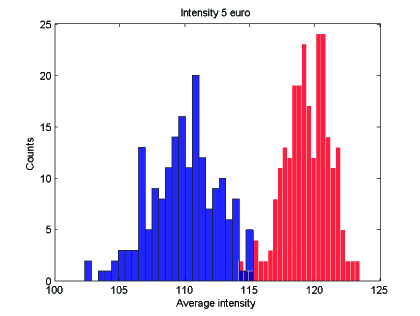
\includegraphics[width=4cm]{img/neur05int.jpg}
						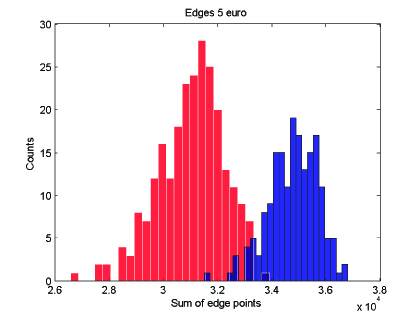
\includegraphics[width=4cm]{img/neur05edge.jpg} \\
						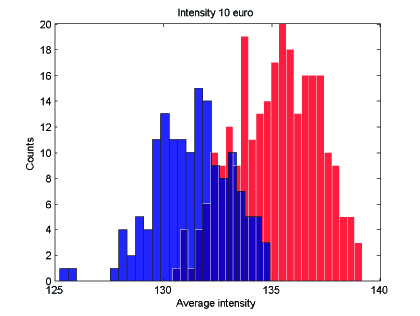
\includegraphics[width=4cm]{img/neur10int.jpg}
						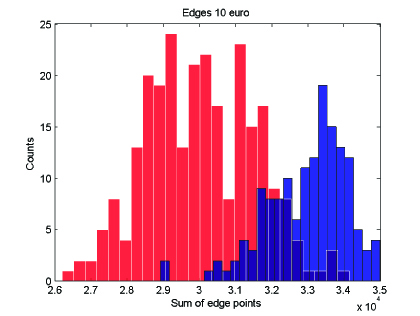
\includegraphics[width=4cm]{img/neur10edge.jpg} \\
					\end{center}
				\end{figure}
		}

		\frame{
			\frametitle{Edges}
			Learning(off-line)
			\begin{itemize}
				\item Perform edge detection on images using Canny edge
				\item Divide edge images into regions
				\item For each region, for each image count the edge points
				\item Calculate Gaussian distribution per region over all images
				\item This results in 2 Gaussian distributions (fit and unfit) for each region
			\end{itemize}
			
			\pause
			Classification (on-line)
			\begin{itemize}
				\item Perform edge detection on incomming image data
				\item Divide edge image into regions
				\item For each region, count the edge points
				\item Calculate probability fit and unfit using gaussian distribution of that region
				\item Classification based on MLE
			\end{itemize}
		}

		\frame{
			\frametitle{Intensity \& edge}
			Learning intensity (off-line)
			\begin{itemize}
				\item Divide images into regions
				\item For each region, for each image calculate average intensity
				\item Calculate Gaussian distribution per region over all images
				\item This results in 2 Gaussian distributions (fit and unfit) for each region
			\end{itemize}
			
			\pause
			Classification intensity (on-line)
			\begin{itemize}
				\item Divide edge image into regions
				\item For each region, calculate average intensity
				\item Calculate probability fit and unfit using gaussian distribution of that region
				\item Classification based on MLE
			\end{itemize}
		}
		
\section{Experiments \& results}
	\frame{
		\frametitle{General setup}
		Holdout set:
		\begin{itemize}
			\item $\approx$ 400 images for both 5 and 10 euro bills
			\item $\approx$ 250 unfit and $\approx$ 150 fit images for both 5 and 10 euro bills
			\item Extract holdout set of 100 images for both
			\item Develop algorithms and train models on the remaining
		\end{itemize}
		\pause
		Training experiment:
		\begin{itemize}
			\item Split remaining data into train-, test- and validation-set
			\item Perform repeated random sub-sampling validation 
			\item Save best performing model over an arbitrary number of repetitions
		\end{itemize}
		
	}
	\frame{
		\frametitle{Results Haar}
		\hspace*{8pt}Haar
	}
	\frame{
		\frametitle{Results PCA}
		\hspace*{8pt}PCA
	}
	\frame{
		\frametitle{Results intensity \& edge}
		\hspace*{8pt}Intensity \& edge
	}
	\frame{
		\frametitle{Results combined}
		\hspace*{8pt}Combined classifier
	}

\section{Conclusion}
	\frame{
		\frametitle{Conclusion}
		\hspace*{8pt}conclusion
	}

\section{future work} 
	\frame{
		\frametitle{Future work}
		\hspace*{8pt}future work
	}
\end{document}

%http://www.dnb.nl/binaries/DNBmag208_tcm46-175321.pdf
